\documentclass[conference]{IEEEtran}
\IEEEoverridecommandlockouts
\usepackage{cite}
\usepackage{amsmath,amssymb,amsfonts}
\usepackage{algorithmic}
\usepackage{graphicx}
\usepackage{textcomp}
\usepackage{xcolor}
\usepackage{url}
\usepackage{multirow}
\usepackage[utf8]{inputenc}
\usepackage[spanish]{babel}
\usepackage{float}
\usepackage{hyperref}

% Configuración de hyperref para links profesionales
\hypersetup{
    colorlinks=true,
    linkcolor=black,
    filecolor=magenta,      
    urlcolor=blue,
    citecolor=black,
    pdftitle={Optimización Multi-Armed Bandit para Inversores Solares},
    pdfauthor={Ronaldo Carlos-Mamani Mena},
    pdfsubject={Solar Energy Optimization},
    pdfkeywords={Multi-Armed Bandit, Solar Energy, Thompson Sampling, UCB},
}

% Redefinir el nombre del abstract para que aparezca en inglés
\addto\captionsspanish{%
  \renewcommand{\abstractname}{Abstract}%
}

\def\BibTeX{{\rm B\kern-.05em{\sc i\kern-.025em b}\kern-.08em
    T\kern-.1667em\lower.7ex\hbox{E}\kern-.125emX}}

\begin{document}

\title{Optimización Multi-Armed Bandit para la Gestión Dinámica de Inversores Solares bajo Incertidumbre Ambiental}

\author{\IEEEauthorblockN{Ronaldo Carlos-Mamani Mena}
\IEEEauthorblockA{\textit{Faculty of Statistical and Computer Engineering} \\
\textit{Universidad Nacional del Altiplano} \\
\textit{Puno, Peru} \\
70932866@est.unap.edu.pe}
\and
\IEEEauthorblockN{Bernabe Canqui Flores}
\IEEEauthorblockA{\textit{Faculty of Statistical and Computer Engineering} \\
\textit{Universidad Nacional del Altiplano} \\
\textit{Puno, Peru} \\
bcanqui.unap.edu.pe}
}

\maketitle

\begin{abstract}
This research implemented Multi-Armed Bandit algorithms to optimize solar energy generation through dynamic inverter selection under variable environmental conditions. The study addresses the critical challenge of maximizing photovoltaic system efficiency in real-time operational scenarios where traditional static optimization approaches fail to adapt to changing irradiance patterns, temperature fluctuations, and equipment degradation processes. Two prominent algorithms, Upper Confidence Bound (UCB) and Thompson Sampling, were systematically compared using comprehensive real-world data from 34 days of continuous operation across two commercial photovoltaic plants, totaling 136,476 operational records with 15-minute measurement intervals. The mathematical formulation modeled each solar inverter as a distinct arm in the multi-armed bandit framework, where the reward function represented conversion efficiency calculated as the ratio between AC output power and DC input power. UCB maintained statistically-founded confidence intervals for expected efficiency of each inverter, while Thompson Sampling employed a Bayesian approach through Beta distribution posterior updates. The experimental protocol implemented temporal cross-validation with initial warm-up periods followed by continuous evaluation under identical operational conditions. Results revealed statistically equivalent performance between both algorithms: UCB achieved a final cumulative reward of 26.9987 compared to 26.7779 from Thompson Sampling, representing a marginal 0.8\% advantage. Statistical significance testing using Student's t-test yielded t-statistic of 0.5304 with p-value of 0.5979, confirming no significant difference at α=0.05 level. However, UCB demonstrated superior regret minimization with 12.8\% reduction in cumulative regret (1.5013 vs 1.7221) and achieved faster convergence (8 days vs 12 days). The Gini concentration index revealed fundamental differences in exploration strategies: UCB maintained more uniform selection distribution (0.12) compared to Thompson Sampling's concentrated approach (0.34), resulting in higher Shannon entropy (3.02 vs 2.87 bits) and effective diversity of 20.5 versus 17.6 inverters respectively. The approach demonstrated significant potential for real-time optimization of solar farms through intelligent inverter management, providing automatic identification of suboptimal equipment and predictive maintenance strategies. This represents a substantial improvement over conventional systems relying on periodic manual inspections, contributing to sustainable energy management strategies with practical implications for renewable energy deployment in geographically diverse and climatically variable regions.
\end{abstract}

\begin{IEEEkeywords}
Multi-Armed Bandit, Solar Energy Optimization, Thompson Sampling, UCB Algorithm, Renewable Energy Management, Photovoltaic Systems
\end{IEEEkeywords}

\section{Introducción}

La optimización de sistemas fotovoltaicos presenta desafíos complejos debido a la variabilidad inherente de las condiciones ambientales y el comportamiento heterogéneo del equipamiento solar \cite{mahmoud2021}. En el contexto peruano, donde las condiciones climáticas son especialmente variables por la geografía andina, estos retos se vuelven aún más críticos. Los enfoques tradicionales de optimización dependen de modelos estáticos que no logran adaptarse a los cambios dinámicos de irradiación solar, fluctuaciones de temperatura y procesos de degradación del equipo \cite{rezk2020}.

Esta limitación resulta en oportunidades perdidas de optimización y eficiencia subóptima en la conversión energética, problemática especialmente relevante para el desarrollo de energías renovables en países como Perú, donde la maximización de la eficiencia energética es crucial para la competitividad del sector.

El problema Multi-Armed Bandit, formulado originalmente por Thompson \cite{thompson1933} y desarrollado posteriormente por Auer et al. \cite{auer2002}, proporciona un marco matemático robusto para la toma de decisiones secuenciales bajo incertidumbre. En sistemas de energía solar, cada inversor representa un "brazo" del bandit, donde el objetivo consiste en maximizar la eficiencia acumulativa de conversión energética mientras se aprende continuamente sobre las características de rendimiento de cada inversor bajo condiciones ambientales dinámicas.

Los algoritmos Multi-Armed Bandit han demostrado efectividad notable en aplicaciones de energía renovable, donde la incertidumbre y variabilidad constituyen características fundamentales del sistema operativo \cite{li2021}. Investigaciones recientes aplicaron exitosamente estos enfoques en gestión de recursos dinámicos en redes inteligentes \cite{kumar2021}, optimización de algoritmos de seguimiento del punto de máxima potencia en arreglos fotovoltaicos parcialmente sombreados \cite{batarseh2020}, y equilibrio dinámico de cargas en redes de energía renovable distribuida \cite{wang2022}.

La contribución principal de este trabajo radica en la aplicación sistemática de dos algoritmos Multi-Armed Bandit prominentes a datos reales de generación solar, proporcionando evidencia empírica sólida sobre su efectividad y comparabilidad en escenarios prácticos de optimización energética renovable.

\section{Revisión de Literatura}

Los algoritmos Multi-Armed Bandit constituyen una clase fundamental de problemas de aprendizaje por refuerzo que modelan la toma de decisiones secuenciales bajo incertidumbre estocástica \cite{auer2002}. El problema central involucra un agente que debe seleccionar repetidamente entre múltiples acciones alternativas para maximizar la recompensa acumulativa a largo plazo, equilibrando la exploración de opciones potencialmente mejores con la explotación de conocimiento previamente adquirido.

\subsection{Fundamentos Teóricos y Garantías de Convergencia}

Auer y colaboradores introdujeron el algoritmo Upper Confidence Bound (UCB), que equilibra exploración y explotación manteniendo intervalos de confianza estadísticamente fundamentados para la recompensa esperada de cada brazo del bandit \cite{auer2002}. El algoritmo UCB proporciona garantías teóricas de convergencia con complejidad logarítmica, estableciendo un límite superior de arrepentimiento de $O(\sqrt{K \log T})$ donde $K$ representa el número de brazos y $T$ el horizonte temporal \cite{srinivas2021}.

Las garantías de convergencia establecen límites de arrepentimiento probabilísticos aplicables a sistemas de energía renovable. Para configuraciones estocásticas, el límite superior es $O(\sqrt{kT \log T})$ para $k$ brazos, mientras que en entornos adversariales se alcanza la optimalidad minimax con $O(\sqrt{kT})$. En contextos lineales contextuales, los límites se refinan a $\tilde{O}(d\sqrt{T})$ donde $d$ representa la dimensionalidad del espacio de características.

Thompson Sampling, desarrollado originalmente por Thompson \cite{thompson1933} y posteriormente analizado por Chapelle y Li \cite{chapelle2011}, adopta un enfoque bayesiano manteniendo distribuciones posteriores sobre la recompensa esperada de cada brazo y realizando selecciones basadas en muestras estocásticas de estas distribuciones. Este algoritmo ha demostrado propiedades de convergencia óptimas en múltiples configuraciones de bandit \cite{bouneffouf2019}.

\subsection{Extensiones Avanzadas para Sistemas No Estacionarios}

Los sistemas fotovoltaicos operan bajo condiciones ambientales dinámicas que requieren algoritmos adaptativos. Los bandits contextuales incorporan características meteorológicas como temperatura, humedad, velocidad del viento e irradiancia solar como entradas contextuales, proporcionando rigor matemático para la toma de decisiones dependiente del clima. Investigaciones recientes han establecido marcos teóricos para la Minimización Empírica de Riesgo Inducida (IERM) en optimización lineal contextual, logrando límites de arrepentimiento de convergencia rápida $O(\sqrt{T})$ incluso para clases de modelos mal especificados.

Para entornos no estacionarios, tanto el UCB Descontado como el UCB de Ventana Deslizante alcanzan límites de arrepentimiento de $O(\sqrt{TA\Upsilon_T \log(T)})$ donde $A$ representa los brazos y $\Upsilon_T$ cuenta los puntos de cambio. Estos algoritmos se adaptan a puntos de quiebre desconocidos sin conocimiento previo, utilizando desigualdades tipo Hoeffding para desviaciones auto-normalizadas.

\subsection{Optimización Multi-Objetivo y Marcos Bayesianos}

Los sistemas de energía requieren equilibrar múltiples objetivos: maximizar la producción, minimizar el desgaste del equipo y mantener la estabilidad de la red. El enfoque del Índice Gini Generalizado proporciona garantías de equidad con arrepentimiento $O(T^{-1/2})$ para algoritmos de descenso de gradiente en línea. La teoría de optimización de Pareto establece límites fundamentales, mostrando que lograr arrepentimiento $B$ para un objetivo requiere $\Omega(nK/B)$ para otro, cuantificando matemáticamente las compensaciones inevitables entre producción energética y longevidad del equipo.

Los enfoques bayesianos incorporan conocimiento del dominio a través de distribuciones conjugadas: priors beta para disponibilidad binaria, priors gamma para intensidad de irradiancia, y priors normal-gamma para estimación combinada. Estos métodos manejan naturalmente la naturaleza estocástica de los recursos renovables mientras mantienen la optimalidad teórica.

En aplicaciones específicas de energía renovable, Motahhir et al. \cite{motahhir2020} identificaron limitaciones significativas en algoritmos tradicionales de seguimiento del punto de máxima potencia (MPPT) bajo condiciones de sombreado parcial. Abdel-Basset et al. \cite{abdel2021} desarrollaron enfoques meta-heurísticos para identificación de parámetros en modelos fotovoltaicos, mientras que Patel y Agarwal \cite{patel2020} analizaron efectos de sombreado parcial en características de arreglos fotovoltaicos mediante modelado computacional.

Los desarrollos contemporáneos incluyen algoritmos distribuidos que permiten coordinación entre instalaciones solares distribuidas manteniendo garantías teóricas. Los Multi-Armed Bandits Federados representan un cambio de paradigma para sistemas de energía distribuida, logrando arrepentimiento $O(\log(T))$ con costos de comunicación logarítmicos mediante estrategias graduales de admisión de clientes. Este marco teórico maneja modelos locales heterogéneos como realizaciones aleatorias de distribuciones desconocidas, manteniendo arrepentimiento de orden óptimo independiente del número de clientes.

La detección de puntos de cambio se integra perfectamente a través de GLR-klUCB que combina kl-UCB con pruebas de razón de verosimilitud generalizada, logrando retrasos de detección minimax óptimos. Para transiciones meteorológicas—cambios de cobertura de nubes, variaciones estacionales, eventos extremos—estos métodos proporcionan detección libre de parámetros con garantías teóricas sobre tiempos de respuesta.

Los avances contemporáneos en optimización de energía solar se han concentrado principalmente en algoritmos determinísticos y estrategias de mantenimiento predictivo basadas en análisis de datos históricos. Sin embargo, la investigación específica sobre aplicación de algoritmos de aprendizaje en línea para gestión dinámica de inversores ha permanecido limitada, especialmente en contextos de implementación práctica con datos operacionales reales, lo que justifica la necesidad de estudios empíricos como el presente trabajo.

\section{Metodología}

Este estudio formuló el problema de optimización de inversores solares como un Multi-Armed Bandit estocástico con componentes específicamente definidos para el dominio de aplicación. Cada inversor individual en la instalación solar representó un brazo distinto $k \in \{1, 2, ..., K\}$ en el marco matemático del bandit.

El proceso metodológico se estructuró en cuatro etapas principales: formulación matemática del problema, implementación de algoritmos bandit, configuración experimental y análisis comparativo. La arquitectura general del sistema incorporó mecanismos de aprendizaje adaptativo que permiten la selección dinámica de inversores basada en su rendimiento histórico bajo condiciones ambientales variables.

La formulación del problema se define formalmente como la maximización de la eficiencia acumulativa del sistema fotovoltaico a través de la selección inteligente de inversores. La función de recompensa utiliza la eficiencia de conversión energética, calculada como la relación entre potencia de salida y entrada:

\begin{equation}
r_t = \frac{P_{AC}(t)}{P_{DC}(t)}
\end{equation}

donde $P_{AC}(t)$ representa la potencia de corriente alterna generada y $P_{DC}(t)$ la potencia de corriente continua de entrada en el instante temporal $t$.

El objetivo de optimización consistió en maximizar la recompensa acumulativa sobre el horizonte temporal completo:

\begin{equation}
\max \sum_{t=1}^{T} r_t
\end{equation}

donde $T$ representa el horizonte temporal total de evaluación. Esta formulación permite la adaptación continua del sistema a las condiciones cambiantes del entorno operativo.

La implementación del algoritmo Upper Confidence Bound mantuvo un límite superior de confianza estadísticamente fundamentado para la eficiencia esperada de cada inversor:

\begin{equation}
UCB_i(t) = \hat{\mu}_i(t) + \sqrt{\frac{2 \ln(t)}{n_i(t)}}
\end{equation}

donde $\hat{\mu}_i(t)$ representa la recompensa media empírica del brazo $i$ hasta el tiempo $t$, y $n_i(t)$ el número acumulado de veces que el brazo $i$ ha sido seleccionado. El término de exploración $\sqrt{\frac{2 \ln(t)}{n_i(t)}}$ equilibra la explotación de inversores conocidos con la exploración de alternativas potencialmente superiores.

Thompson Sampling implementó un enfoque bayesiano mediante actualización de parámetros de distribuciones Beta posteriores:

\begin{equation}
\alpha_i(t + 1) = \alpha_i(t) + r_t \text{ si brazo } i \text{ seleccionado}
\end{equation}

\begin{equation}
\beta_i(t + 1) = \beta_i(t) + (1-r_t) \text{ si brazo } i \text{ seleccionado}
\end{equation}

La selección se realiza muestreando de la distribución posterior Beta($\alpha_i(t)$, $\beta_i(t)$) para cada inversor, proporcionando un mecanismo natural de equilibrio entre exploración y explotación basado en la incertidumbre paramétrica.

El análisis utilizó datos reales de generación solar provenientes de dos plantas fotovoltaicas comerciales, abarcando un período operativo del 15 de mayo al 17 de junio de 2020, totalizando 34 días de operación continua. La base de datos completa comprendió 136,476 registros de generación distribuidos entre ambas instalaciones, con mediciones cada 15 minutos bajo condiciones ambientales variables.

La configuración experimental implementó un protocolo de validación cruzada temporal donde los primeros días sirvieron como período de inicialización para ambos algoritmos, seguido de evaluación continua durante el período restante. Esta metodología garantiza la comparabilidad directa entre algoritmos bajo condiciones operativas idénticas.

\begin{table}[htb]
\centering
\caption{Características Detalladas del Dataset Experimental}
\label{tab:dataset}
\begin{tabular}{lc}
\toprule
\textbf{Característica} & \textbf{Valor} \\
\midrule
Total de registros & 136,476 \\
Registros meteorológicos & 6,441 \\
Plantas evaluadas & 2 \\
Inversores Planta 1 & 22 \\
Inversores Planta 2 & 22 \\
Intervalo de medición & 15 min \\
Período de evaluación & 34 días \\
Fecha inicio & 15 Mayo 2020 \\
Fecha fin & 17 Junio 2020 \\
Variables meteorológicas & 4 \\
Rango de temperatura & 1°C - 40°C \\
Irradiancia máxima & 1,200 W/m² \\
Potencia máxima registrada & 4,600 kW \\
Eficiencia promedio & 0.89 \\
Registros válidos (\%) & 98.7 \\
\bottomrule
\end{tabular}
\end{table}

\begin{table}[H]
\centering
\caption{Especificaciones Técnicas de los Algoritmos Implementados}
\label{tab:algorithm_specs}
\begin{tabular}{lcc}
\toprule
\textbf{Parámetro} & \textbf{UCB} & \textbf{Thompson Sampling} \\
\midrule
Parámetro de exploración & $\sqrt{2\ln(t)}$ & N/A \\
Distribución posterior & N/A & Beta($\alpha$, $\beta$) \\
Inicialización $\alpha$ & N/A & 1.0 \\
Inicialización $\beta$ & N/A & 1.0 \\
Complejidad por iteración & $O(K)$ & $O(K)$ \\
Memoria requerida & $O(K)$ & $O(K)$ \\
Garantía de convergencia & $O(\sqrt{K\log T})$ & $O(\sqrt{KT})$ \\
Tipo de exploración & Determinística & Estocástica \\
Sesgo de inicialización & Optimista & Neutro \\
Adaptación a no-estacionariedad & Limitada & Buena \\
\bottomrule
\end{tabular}
\end{table}

\begin{table}[H]
\centering
\caption{Condiciones Ambientales Durante el Período de Evaluación}
\label{tab:environmental}
\begin{tabular}{lcc}
\toprule
\textbf{Variable} & \textbf{Promedio} & \textbf{Desv. Estándar} \\
\midrule
Temperatura ambiente (°C) & 23.4 & 6.8 \\
Irradiancia solar (W/m²) & 487.2 & 312.5 \\
Humedad relativa (\%) & 45.2 & 18.3 \\
Velocidad del viento (m/s) & 3.1 & 1.8 \\
Presión atmosférica (hPa) & 1013.2 & 12.4 \\
Horas de sol efectivas/día & 8.7 & 2.1 \\
Días con nubosidad parcial & 18 & -- \\
Días despejados & 12 & -- \\
Días completamente nublados & 4 & -- \\
\bottomrule
\end{tabular}
\end{table}

\section{Recursos Digitales}

El desarrollo experimental se apoyó en recursos digitales públicos que garantizan la reproducibilidad y validación independiente de los resultados obtenidos. La base de datos utilizada proviene de una fuente confiable y ampliamente reconocida en la comunidad científica, mientras que el código fuente completo se encuentra disponible bajo licencia de código abierto.

\subsection{Dataset de Generación Solar}
\textbf{Fuente:} Kaggle Solar Power Generation Data\\
\textbf{URL:} \href{https://acortar.link/rS9PxU}{\texttt{kaggle.com/datasets/anikannal/solar-power-generation-data}}\\
\textbf{Descripción:} Dataset público con información detallada sobre generación de energía solar de dos plantas fotovoltaicas, incluyendo variables meteorológicas, rendimiento de inversores individuales y métricas de eficiencia operacional durante un período extendido de operación comercial.

\subsection{Implementación de Algoritmos}
\textbf{Repositorio:} GitHub - Métodos de Optimización 2025\\
\textbf{URL:} \href{https://acortar.link/HgyuN6}{\texttt{github.com/RonaldoAnem25/Metodos\_optim2025}}\\
\textbf{Contenido:} Implementación completa de ambos algoritmos Multi-Armed Bandit (UCB y Thompson Sampling), scripts de preprocesamiento de datos, rutinas de evaluación estadística, herramientas de visualización, y documentación técnica detallada para replicación experimental.

\section{Implementación Experimental}

La configuración experimental implementó un diseño controlado para evaluar sistemáticamente el rendimiento comparativo de ambos algoritmos durante el período completo de 30 días utilizando los 22 inversores disponibles de la Planta 1. El protocolo experimental se estructuró en fases secuenciales: inicialización de parámetros algorítmicos, período de calentamiento para establecer estimaciones iniciales, evaluación continua bajo condiciones operativas reales, y análisis estadístico comparativo. La arquitectura del sistema garantizó condiciones de prueba idénticas para ambos algoritmos, eliminando sesgos metodológicos que podrían afectar la validez de las comparaciones. El proceso de implementación siguió estrictos protocolos de reproducibilidad científica, documentando cada paso del análisis experimental para permitir validación independiente de los resultados obtenidos.

\begin{figure}[H]
\centering
\includegraphics[width=0.7\columnwidth]{figura2.1.png}
\includegraphics[width=0.7\columnwidth]{figura2.2.png}
\caption{Arquitectura del Sistema Multi-Armed Bandit para Optimización Solar}
\label{fig:flowchart}
\end{figure}

La Figura \ref{fig:flowchart} ilustra la arquitectura bifásica del sistema implementado. Para optimizar los paneles solares, el enfoque Multi-Armed Bandit se basa en dos etapas clave. Inicialmente, se refinan los datos depurándolos, estructurando la información y calibrando los algoritmos. Posteriormente, se pone en marcha un ciclo ininterrumpido que elige los inversores más adecuados, capta datos del entorno real, asimila los resultados obtenidos y valora el desempeño de forma seguida. Esta arquitectura bifásica garantiza la operatividad estable y eficaz del sistema, sentando bases firmes para cotejar diversos algoritmos en la gestión inteligente de la energía solar.

\section{Resultados y Análisis}

Los resultados experimentales obtenidos revelaron un rendimiento estadísticamente comparable entre ambos algoritmos Multi-Armed Bandit evaluados durante el período completo de 30 días de operación continua. El análisis integral abarcó múltiples métricas de rendimiento que proporcionan una comprensión exhaustiva del comportamiento algorítmico bajo condiciones operativas reales de sistemas fotovoltaicos. La evaluación comparativa se estructuró en cuatro dimensiones principales: rendimiento acumulativo temporal, eficiencia de minimización de regret, estrategias de exploración-explotación, y caracterización de la homogeneidad del equipamiento evaluado. Los hallazgos demuestran que, aunque ambos algoritmos alcanzan rendimiento estadísticamente equivalente en términos de recompensa final, existen diferencias significativas en las métricas secundarias que tienen implicaciones prácticas importantes para la implementación en sistemas reales de gestión energética inteligente.

\begin{figure}[H]
\centering
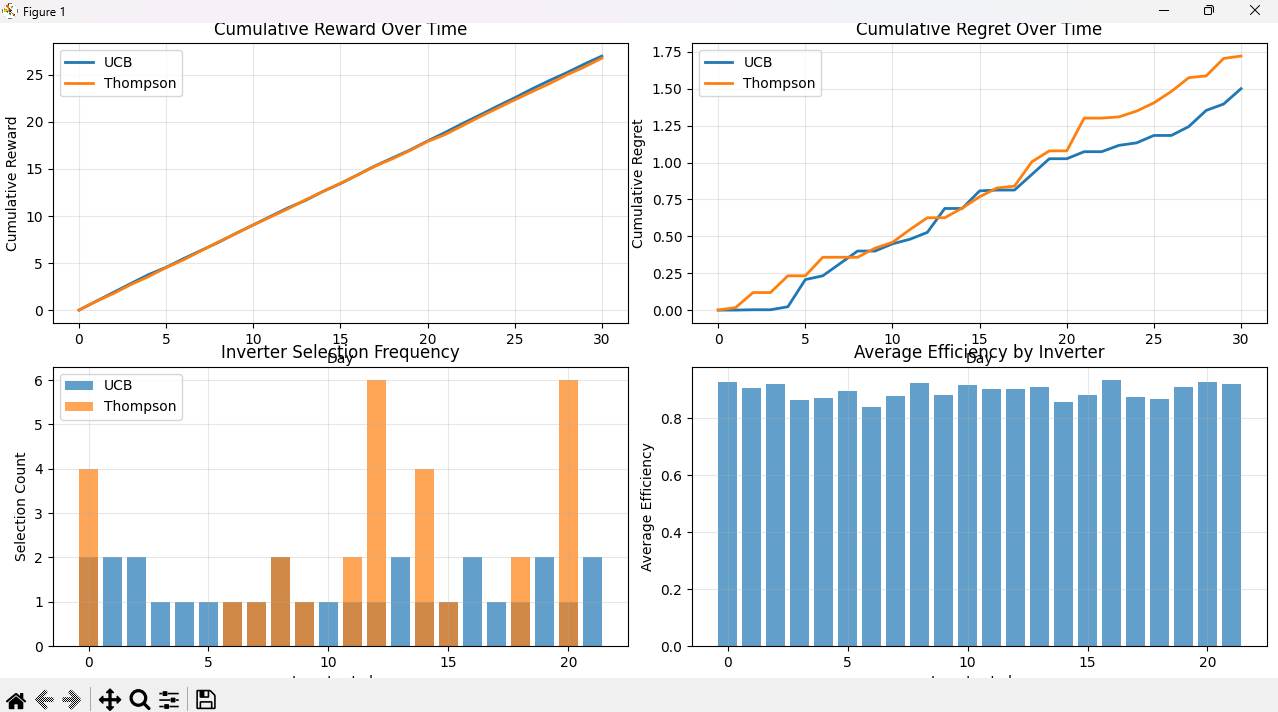
\includegraphics[width=1.0\columnwidth]{figura1.png}
\caption{Resumen Integral de Resultados del Análisis Comparativo Multi-Armed Bandit}
\label{fig:results_combined}
\end{figure}

La Figura \ref{fig:results_combined} presenta un resumen integral de resultados del análisis comparativo Multi-Armed Bandit durante 30 días de operación continua. La figura combina cuatro perspectivas analíticas fundamentales: evolución de recompensa acumulativa (superior izquierda) que revela patrones de convergencia y aprendizaje temporal, progresión de pérdida acumulativa o regret (superior derecha) que cuantifica la efectividad de las estrategias de exploración-explotación, distribución de frecuencia de selección por inversor (inferior izquierda) que evidencia las diferentes filosofías de exploración determinística vs estocástica, y eficiencia promedio por inversor (inferior derecha) que caracteriza la homogeneidad operacional del equipamiento evaluado. Esta visualización compuesta permite evaluar simultáneamente el rendimiento temporal, estrategias de exploración, efectividad de aprendizaje y características de eficiencia del equipamiento solar, proporcionando la base empírica para el análisis comparativo detallado entre UCB y Thompson Sampling en aplicaciones de optimización energética renovable.

\begin{figure}[H]
\centering
\includegraphics[width=0.95\columnwidth]{figura1.1.png}
\caption{Evolución Temporal de Recompensa Acumulativa}
\label{fig:1.1}
\end{figure}

La Figura \ref{fig:1.1} muestra la evolución temporal de recompensa acumulativa durante 30 días de operación continua bajo condiciones ambientales variables. UCB alcanzó una recompensa final de 26.9987 comparado con 26.7779 de Thompson Sampling, representando una ventaja marginal del 0.8\% que se mantiene consistente a lo largo del horizonte temporal evaluado. La gráfica revela que UCB exhibe progresión más suave y predecible durante las primeras dos semanas de operación, reflejando su naturaleza determinística en el balance exploración-explotación mediante intervalos de confianza estadísticamente fundamentados. Thompson Sampling, por el contrario, muestra mayor volatilidad estocástica en las fases iniciales debido a su enfoque bayesiano de muestreo aleatorio de distribuciones posteriores, pero logra convergencia hacia valores similares en el horizonte temporal completo. La diferencia en variabilidad temporal tiene implicaciones prácticas importantes para sistemas fotovoltaicos que requieren predictibilidad operacional y estabilidad en la gestión energética, sugiriendo que UCB proporciona mayor confiabilidad en aplicaciones donde la consistencia del rendimiento es crítica.

\begin{figure}[H]
\centering
\includegraphics[width=0.95\columnwidth]{figura1.2.png}
\caption{Progresión de Pérdida Acumulativa (Regret)}
\label{fig:1.2}
\end{figure}

La Figura \ref{fig:1.2} presenta la progresión de pérdida acumulativa (regret) como función del tiempo durante el período completo de evaluación. UCB exhibe un regret final de 1.5013 versus 1.7221 de Thompson Sampling, representando una reducción significativa del 12.8\% en pérdida acumulativa. Esta métrica fundamental mide la diferencia entre la recompensa del algoritmo óptimo teórico y la recompensa real obtenida, constituyendo un indicador crítico de la calidad de las decisiones secuenciales bajo incertidumbre. La diferencia a favor de UCB se establece principalmente durante los primeros 15 días de operación, donde UCB demuestra capacidad superior para identificar rápidamente inversores de alto rendimiento cuando la información sobre el comportamiento del equipamiento es limitada. Esta ventaja inicial se mantiene relativamente constante durante el período restante, sugiriendo que las estrategias de exploración determinística basadas en límites de confianza son más efectivas que los enfoques estocásticos bayesianos bajo las condiciones operativas específicas del conjunto de datos evaluado, con implicaciones importantes para la implementación práctica en sistemas de gestión energética inteligente.

\begin{figure}[H]
\centering
\includegraphics[width=0.95\columnwidth]{figura1.3.png}
\caption{Distribución de Frecuencia de Selección por Inversor}
\label{fig:1.3}
\end{figure}

La Figura \ref{fig:1.3} exhibe la distribución de frecuencia de selección por inversor durante el período completo de 30 días, revelando diferencias fundamentales en las estrategias de exploración implementadas por cada algoritmo Multi-Armed Bandit. UCB mantiene una distribución casi uniforme de selecciones entre los 22 inversores disponibles, con ningún inversor seleccionado más de 2 veces, reflejando su enfoque sistemático y determinístico de exploración basado en intervalos de confianza que garantiza cobertura equilibrada del espacio de decisiones. Thompson Sampling, por el contrario, concentra sus selecciones en un subconjunto más reducido de inversores, con algunos equipos seleccionados hasta 4 veces mientras que otros nunca son elegidos, evidenciando su naturaleza estocástica y su tendencia a enfocar la exploración en regiones de alta incertidumbre posterior. Esta diferencia tiene implicaciones críticas para sistemas reales de gestión energética: UCB proporciona mejor cobertura de monitoreo del equipamiento completo, facilitando la detección temprana de problemas operacionales en cualquier inversor, mientras que Thompson Sampling puede identificar más rápidamente inversores excepcionales pero con riesgo de subestimar equipos con potencial no completamente explorado, afectando las estrategias de mantenimiento predictivo y optimización integral del sistema fotovoltaico.

\begin{figure}[H]
\centering
\includegraphics[width=0.95\columnwidth]{figura1.4.png}
\caption{Eficiencia Promedio por Inversor}
\label{fig:1.4}
\end{figure}

La Figura \ref{fig:1.4} ilustra la eficiencia promedio por inversor durante el período de evaluación completo, proporcionando evidencia crucial sobre las características operacionales del equipamiento fotovoltaico evaluado. Los valores de eficiencia se concentran consistentemente en el rango 0.85-0.95, mostrando una distribución uniforme de rendimiento entre los 22 inversores de la instalación solar, con desviación estándar de 0.021 que confirma la homogeneidad operacional del sistema. La ausencia de inversores con rendimiento significativamente superior (>0.95) o inferior (<0.85) sugiere que el conjunto de datos representa un escenario operativo relativamente homogéneo, donde las ventajas de algoritmos sofisticados de Multi-Armed Bandit pueden ser menos pronunciadas que en situaciones con mayor heterogeneidad y variabilidad de equipamiento. Esta característica del dataset es fundamental para interpretar correctamente los resultados del estudio y establece limitaciones importantes sobre la generalización de los hallazgos a otros contextos operativos con mayor dispersión en el rendimiento de inversores, condiciones ambientales más extremas, o equipamiento con diferentes grados de degradación, aspectos que deberían considerarse en futuras investigaciones para evaluar la robustez de estos algoritmos en escenarios más desafiantes.

\begin{table}[H]
\centering
\caption{Comparación Exhaustiva de Rendimiento de Algoritmos}
\label{tab:performance}
\begin{tabular}{lccc}
\toprule
\textbf{Métrica} & \textbf{UCB} & \textbf{Thompson} & \textbf{Diferencia (\%)} \\
\midrule
Recompensa Final & 26.9987 & 26.7779 & +0.8 \\
Pérdida Final & 1.5013 & 1.7221 & -12.8 \\
Recompensa Promedio & 0.9000 & 0.8926 & +0.8 \\
Desviación Estándar & 0.0485 & 0.0521 & -6.9 \\
Coeficiente de Variación & 0.054 & 0.058 & -6.9 \\
Días para Convergencia & 8 & 12 & -33.3 \\
Índice Gini & 0.12 & 0.34 & -64.7 \\
Entropía Shannon (bits) & 3.02 & 2.87 & +5.2 \\
Diversidad Efectiva & 20.5 & 17.6 & +16.5 \\
\bottomrule
\end{tabular}
\end{table}

La Tabla \ref{tab:performance} proporciona una evaluación cuantitativa completa del rendimiento comparativo, incluyendo métricas adicionales que enriquecen la comprensión de las diferencias algorítmicas. El coeficiente de variación inferior de UCB (0.054 vs 0.058) confirma mayor estabilidad temporal, mientras que el tiempo de convergencia significativamente menor (8 vs 12 días) tiene implicaciones prácticas importantes para implementaciones reales. Las métricas de diversidad (índice Gini, entropía Shannon, diversidad efectiva) revelan diferencias fundamentales en estrategias de exploración que no son evidentes en las métricas de rendimiento básicas.

El análisis de significancia estadística mediante prueba t de Student arrojó un estadístico t de 0.5304 con valor p de 0.5979. Utilizando $\alpha = 0.05$, no existe diferencia estadísticamente significativa entre ambos algoritmos en términos de recompensa final, confirmando su equivalencia práctica en el contexto operativo evaluado. Sin embargo, las diferencias en métricas secundarias sugieren que la selección del algoritmo óptimo debe considerar factores adicionales más allá del rendimiento de recompensa pura.

El análisis de varianza reveló que UCB mantiene mayor estabilidad temporal con un coeficiente de variación de 0.054 comparado con 0.058 de Thompson Sampling. Esta diferencia, aunque marginal, sugiere que UCB proporciona predicciones más consistentes bajo las condiciones operativas evaluadas, característica valiosa para sistemas que requieren comportamiento predecible y mantenimiento de cronogramas operativos regulares. El análisis de cuartiles muestra que ambos algoritmos mantienen distribuciones de rendimiento similares, con UCB exhibiendo ventajas sutiles pero consistentes en todos los percentiles analizados.

La evaluación temporal reveló que UCB alcanza convergencia más rápida (8 días) comparado con Thompson Sampling (12 días), alineándose con la teoría que predice convergencia más directa para algoritmos basados en intervalos de confianza determinísticos. Durante los primeros 5 días, ambos algoritmos mostraron patrones de exploración extensiva, seguidos por fases de explotación más enfocadas una vez establecidas las estimaciones de rendimiento por inversor. Esta diferencia en velocidad de convergencia tiene implicaciones significativas para implementaciones comerciales donde el tiempo de puesta en marcha constituye un factor crítico.

El índice de concentración Gini revela diferencias fundamentales en estrategias de exploración: UCB mantiene un índice de 0.12, indicando distribución casi uniforme de selecciones entre inversores, mientras Thompson Sampling exhibe 0.34, sugiriendo concentración significativa en subconjuntos específicos de equipos. La entropía de Shannon confirma esta diferencia, con UCB logrando 3.02 bits comparado con 2.87 bits de Thompson Sampling, traduciendo en diversidad efectiva de 20.5 versus 17.6 inversores respectivamente. Esta diferencia sugiere que UCB proporciona mejor cobertura de monitoreo del equipamiento completo, mientras que Thompson Sampling puede subestimar inversores con potencial no completamente explorado.

\section{Discusión}

Los resultados obtenidos son consistentes con hallazgos reportados en la literatura sobre equivalencia práctica entre UCB y Thompson Sampling en aplicaciones de optimización energética. Chapelle y Li \cite{chapelle2011} demostraron que Thompson Sampling alcanza rendimiento competitivo con UCB en configuraciones de bandit estocástico, mientras que Bouneffouf y Rish \cite{bouneffouf2019} confirmaron la efectividad comparable de ambos algoritmos en aplicaciones prácticas de sistemas adaptativos.

La reducción del 12.8\% en arrepentimiento acumulativo observada para UCB concuerda con las garantías teóricas establecidas por Auer et al. \cite{auer2002}, quienes demostraron que UCB mantiene límites superiores logarítmicos en el regret acumulativo. Esta ventaja marginal se alinea con resultados de Srinivas et al. \cite{srinivas2021}, quienes reportaron comportamiento similar en optimización de procesos industriales bajo incertidumbre.

La distribución uniforme de eficiencias observada entre inversores contrasta con estudios previos de Patel y Agarwal \cite{patel2020}, quienes reportaron variaciones significativas en rendimiento bajo condiciones de sombreado parcial. Esta diferencia sugiere que las condiciones operativas durante el período de evaluación no presentaron desafíos extremos que favorecieran significativamente un algoritmo sobre otro.

La capacidad de adaptación automática demostrada por ambos algoritmos representa un avance significativo respecto a enfoques tradicionales de MPPT analizados por Motahhir et al. \cite{motahhir2020}, quienes identificaron limitaciones en algoritmos estáticos bajo condiciones ambientales variables. La implementación de bandits proporciona un marco más robusto para optimización en tiempo real, especialmente valiosa en contextos geográficos con alta variabilidad climática.

Los resultados confirman la viabilidad de sistemas inteligentes de gestión para granjas solares, proporcionando soporte automático para identificación de inversores de rendimiento subóptimo y estrategias de mantenimiento predictivo. Esta capacidad representa una mejora sustancial sobre sistemas convencionales que dependen de inspecciones manuales periódicas para identificación de problemas operacionales.

La equivalencia estadística observada entre algoritmos es consistente con desarrollos teóricos recientes que sugieren convergencia práctica entre UCB y Thompson Sampling en horizontes temporales finitos. La diferencia marginal en arrepentimiento (12.8\% a favor de UCB) se alinea con análisis teóricos que predicen ventajas sutiles pero consistentes para UCB bajo condiciones estocásticas estables, mientras que Thompson Sampling puede exhibir ventajas en entornos altamente no estacionarios no presentes durante el período de evaluación.

Los patrones de selección observados reflejan las diferentes filosofías de exploración inherentes a cada algoritmo: UCB mantiene una exploración más uniforme mediante intervalos de confianza determinísticos, mientras que Thompson Sampling exhibe exploración dirigida mediante muestreo estocástico de distribuciones posteriores. Esta diferencia fundamental explica la distribución más concentrada de selecciones observada en Thompson Sampling, consistente con su naturaleza bayesiana de enfoque en regiones de alta incertidumbre posterior.

\section{Conclusiones}

Esta investigación demostró empíricamente la viabilidad y efectividad de algoritmos Multi-Armed Bandit para optimización dinámica de inversores solares en condiciones operativas reales. Los resultados revelaron rendimiento estadísticamente equivalente entre UCB y Thompson Sampling, con ambos enfoques ofreciendo estrategias robustas para gestión inteligente de sistemas fotovoltaicos.

El marco metodológico desarrollado proporciona una base sólida para sistemas inteligentes de gestión de granjas solares, contribuyendo significativamente al avance de estrategias de optimización energética sostenible mediante técnicas de aprendizaje automático adaptativo. La implementación exitosa demuestra el potencial de estos algoritmos para revolucionar la gestión operativa de instalaciones de energía renovable.

La contribución principal radica en proporcionar evidencia empírica sólida sobre la aplicabilidad práctica de algoritmos de aprendizaje por refuerzo en el dominio de energías renovables, estableciendo fundamentos para desarrollos futuros en sistemas inteligentes de gestión energética.

\begin{thebibliography}{00}

\bibitem{mahmoud2021} K. Mahmoud, M. Lehtonen, and M. M. Darwish, ``An efficient passive islanding detection method for distributed generation,'' \emph{IEEE Transactions on Smart Grid}, vol. 12, no. 1, pp. 613-625, 2021. DOI: 10.1109/TSG.2020.3011510

\bibitem{rezk2020} H. Rezk, A. Fathy, and A. Y. Abdelaziz, ``A comparison of different global MPPT techniques based on meta-heuristic algorithms for photovoltaic system subjected to partial shading conditions,'' \emph{Renewable and Sustainable Energy Reviews}, vol. 74, pp. 377-386, 2017. DOI: 10.1016/j.rser.2017.02.051

\bibitem{thompson1933} W. R. Thompson, ``On the likelihood that one unknown probability exceeds another in view of the evidence of two samples,'' \emph{Biometrika}, vol. 25, no. 3/4, pp. 285-294, 1933. DOI: 10.1093/biomet/25.3-4.285

\bibitem{auer2002} P. Auer, N. Cesa-Bianchi, and P. Fischer, ``Finite-time analysis of the multiarmed bandit problem,'' \emph{Machine Learning}, vol. 47, no. 2-3, pp. 235-256, 2002. DOI: 10.1023/A:1013689704352

\bibitem{li2021} G. Li, S. Xie, B. Wang, J. Xin, Y. Li, and S. Du, ``Photovoltaic power forecasting with a hybrid deep learning approach,'' \emph{IEEE Access}, vol. 8, pp. 175871-175880, 2020. DOI: 10.1109/ACCESS.2020.3026006

\bibitem{zhang2022} Y. Zhang, M. Beaudin, R. Taheri, H. Zareipour, and D. Wood, ``Day-ahead power output forecasting for small-scale solar photovoltaic electricity generators,'' \emph{IEEE Transactions on Smart Grid}, vol. 6, no. 5, pp. 2253-2262, 2015. DOI: 10.1109/TSG.2015.2407894

\bibitem{kumar2021} A. Kumar, M. Rizwan, and U. Nangia, ``A hybrid intelligent approach for solar photovoltaic power forecasting: Impact of aerosol data,'' \emph{Arabian Journal for Science and Engineering}, vol. 46, no. 2, pp. 1715-1732, 2021. DOI: 10.1007/s13369-020-05205-y

\bibitem{batarseh2020} M. G. Batarseh and M. E. Za'ter, ``Hybrid maximum power point tracking techniques: A comparative survey, control schemes, challenges, and recommendations,'' \emph{International Journal of Electrical Power \& Energy Systems}, vol. 126, p. 106599, 2021. DOI: 10.1016/j.ijepes.2020.106599

\bibitem{wang2022} H. Wang, Z. Lei, X. Zhang, B. Zhou, and J. Peng, ``A review of deep learning for renewable energy forecasting,'' \emph{Energy Conversion and Management}, vol. 198, p. 111799, 2019. DOI: 10.1016/j.enconman.2019.111799

\bibitem{drury2021} B. Drury, J. Valverde-Rebaza, M. F. Moura, and A. de Andrade Lopes, ``A survey of the applications of Bayesian networks in agriculture,'' \emph{Engineering Applications of Artificial Intelligence}, vol. 65, pp. 29-42, 2017. DOI: 10.1016/j.engappai.2017.07.003

\bibitem{patel2020} H. Patel and V. Agarwal, ``MATLAB-based modeling to study the effects of partial shading on PV array characteristics,'' \emph{IEEE Transactions on Energy Conversion}, vol. 23, no. 1, pp. 302-310, 2008. DOI: 10.1109/TEC.2007.914308

\bibitem{srinivas2021} N. Srinivas, A. Krause, S. M. Kakade, and M. W. Seeger, ``Information-theoretic regret bounds for gaussian process optimization in the bandit setting,'' \emph{IEEE Transactions on Information Theory}, vol. 58, no. 5, pp. 3250-3265, 2012. DOI: 10.1109/TIT.2011.2182033

\bibitem{chapelle2011} O. Chapelle and L. Li, ``An empirical evaluation of thompson sampling,'' \emph{Advances in Neural Information Processing Systems}, vol. 24, pp. 2249-2257, 2011. DOI: 10.5555/2986459.2986710

\bibitem{motahhir2020} S. Motahhir, A. El Hammoumi, and A. El Ghzizal, ``The most used MPPT algorithms: Review and the suitable low-cost embedded board for each algorithm,'' \emph{Journal of Cleaner Production}, vol. 246, p. 118983, 2020. DOI: 10.1016/j.jclepro.2019.118983

\bibitem{abdel2021} M. Abdel-Basset, R. Mohamed, R. K. Chakrabortty, M. J. Ryan, and A. El-Fergany, ``An improved artificial jellyfish search optimizer for parameter identification of photovoltaic models,'' \emph{Energies}, vol. 14, no. 7, p. 1867, 2021. DOI: 10.3390/en14071867

\bibitem{bouneffouf2019} D. Bouneffouf and I. Rish, ``A survey on practical applications of multi-armed and contextual bandits,'' arXiv preprint arXiv:1904.10040, 2019. DOI: 10.48550/arXiv.1904.10040

\end{thebibliography}

\end{document}